\chapter{Data Sharing}

To share data, you will create a guest collection and grant your collaborators access as described in the instructions below. If you like, you can designate other Globus users as "access managers" for the guest collection, allowing them to grant or revoke access privileges for other Globus users.

\begin{center}
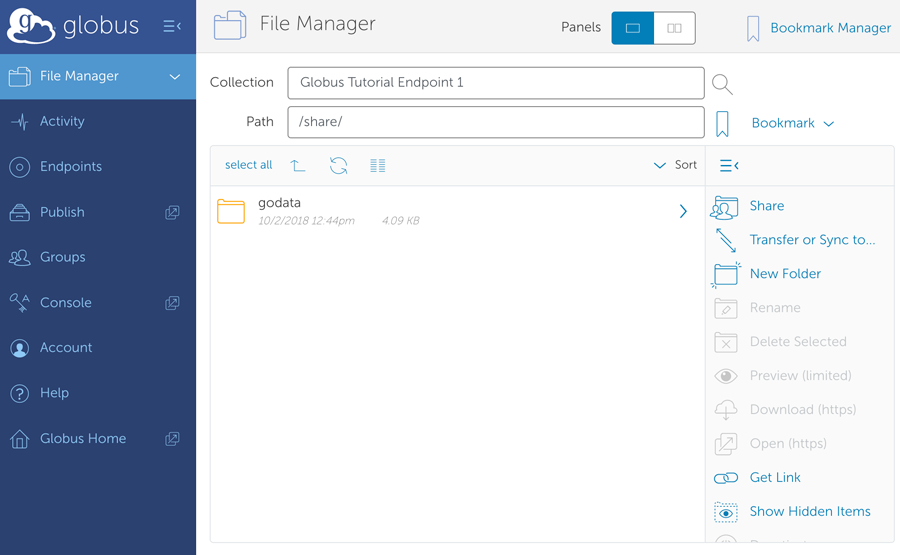
\includegraphics[width=0.5\textwidth]{img/sharedata-1.png}
\end{center}

\begin{itemize}
\item Login to Globus and navigate to emph{File Manager}.
\item Select the collection that has the files/folders you wish to share and, if necessary, activate the collection.
\item Highlight the folder that you would like to share and click \emph{Share} in the right command panel.
\item If \emph{Share} is not available, contact the endpoint’s administrator or refer to \href{https://docs.globus.org/globus-connect-server-installation-guide/}{Globus Connect Server Installation Guide} for instructions on enabling sharing. If you are a using a \gls{Globus Connect} Personal endpoint and you are a Globus Plus user, enable sharing by opening the Preferences for \gls{Globus Connect} Personal, clicking the \emph{Access} tab, and checking the Sharable box.
\item Provide a name for the guest collection, and click \emph{Create Share}.
\item When your collection is created, you will be taken to the Sharing tab, where you can set permissions. As shown below, the starting permissions give read and write access (and the Administrator role) to the person who created the collection.
Click the \emph{Add Permissions} button or icon to share access with others. You can add permissions for an individual user, for a \href{https://docs.globus.org/how-to/managing-groups/}{group}, or for all logged-in users. In the \emph{Identity/E-mail} field, type a person's name or username (if user is selected) or a group name (if group is selected) and press \emph{Enter}. Globus will display matching identities. Pick from the list. If the user has not used Globus before or you only have an email address, enter the email address and click \emph{Add}.
The users you share with will receive an email notification containing a link to the shared endpoint. You may add a customized message to this email. If you do not want to send a notification, uncheck the \emph{Send E-mail} checkbox.
You can add permissions to subfolders by entering a path in the \emph{Path} field.
\item After receiving the email notification, your colleague can click on the link to log into Globus and access the guest collection.
\item You can allow others to manage the permissions for a collection you create. Use the \emph{Roles} tab to manage roles for other users. You can assign roles to individual users or to groups. As shown below, the default is for the person who created the collection to have the Administrator role.
The Access Manager role grants the ability to manage permissions for a collection. (Users with this role automatically have read/write access for the collection.)
When a role is assigned to a group, all members of the group have the assigned role.
\end{itemize}

%%% Local Variables:
%%% mode: latex
%%% TeX-master: "intro-Globus"
%%% End:
